%% Based on a TeXnicCenter-Template by Tino Weinkauf.
%%%%%%%%%%%%%%%%%%%%%%%%%%%%%%%%%%%%%%%%%%%%%%%%%%%%%%%%%%%%%

%%%%%%%%%%%%%%%%%%%%%%%%%%%%%%%%%%%%%%%%%%%%%%%%%%%%%%%%%%%%%
%% HEADER
%%%%%%%%%%%%%%%%%%%%%%%%%%%%%%%%%%%%%%%%%%%%%%%%%%%%%%%%%%%%%
\documentclass[a4paper,10pt]{report}
% Alternative Options:
%	Paper Size: a4paper / a5paper / b5paper / letterpaper / legalpaper / executivepaper
% Duplex: oneside / twoside
% Base Font Size: 10pt / 11pt / 12pt


%% Language %%%%%%%%%%%%%%%%%%%%%%%%%%%%%%%%%%%%%%%%%%%%%%%%%
\usepackage[USenglish]{babel} %francais, polish, spanish, ...
\usepackage[T1]{fontenc}
\usepackage[ansinew]{inputenc}

\usepackage{lmodern} %Type1-font for non-english texts and characters


%% Packages for Graphics & Figures %%%%%%%%%%%%%%%%%%%%%%%%%%
\usepackage{graphicx} %%For loading graphic files
%\usepackage{subfig} %%Subfigures inside a figure
%\usepackage{tikz} %%Generate vector graphics from within LaTeX

%% Please note:
%% Images can be included using \includegraphics{filename}
%% resp. using the dialog in the Insert menu.
%% 
%% The mode "LaTeX => PDF" allows the following formats:
%%   .jpg  .png  .pdf  .mps
%% 
%% The modes "LaTeX => DVI", "LaTeX => PS" und "LaTeX => PS => PDF"
%% allow the following formats:
%%   .eps  .ps  .bmp  .pict  .pntg


%% Math Packages %%%%%%%%%%%%%%%%%%%%%%%%%%%%%%%%%%%%%%%%%%%%
\usepackage{amsmath}
\usepackage{amsthm}
\usepackage{amsfonts}


%% Line Spacing %%%%%%%%%%%%%%%%%%%%%%%%%%%%%%%%%%%%%%%%%%%%%
%\usepackage{setspace}
%\singlespacing        %% 1-spacing (default)
%\onehalfspacing       %% 1,5-spacing
%\doublespacing        %% 2-spacing


%% Other Packages %%%%%%%%%%%%%%%%%%%%%%%%%%%%%%%%%%%%%%%%%%%
%\usepackage{a4wide} %%Smaller margins = more text per page.
%\usepackage{fancyhdr} %%Fancy headings
%\usepackage{longtable} %%For tables, that exceed one page


%%%%%%%%%%%%%%%%%%%%%%%%%%%%%%%%%%%%%%%%%%%%%%%%%%%%%%%%%%%%%
%% Remarks
%%%%%%%%%%%%%%%%%%%%%%%%%%%%%%%%%%%%%%%%%%%%%%%%%%%%%%%%%%%%%
%
% TODO:
% 1. Edit the used packages and their options (see above).
% 2. If you want, add a BibTeX-File to the project
%    (e.g., 'literature.bib').
% 3. Happy TeXing!
%
%%%%%%%%%%%%%%%%%%%%%%%%%%%%%%%%%%%%%%%%%%%%%%%%%%%%%%%%%%%%%

%%%%%%%%%%%%%%%%%%%%%%%%%%%%%%%%%%%%%%%%%%%%%%%%%%%%%%%%%%%%%
%% Options / Modifications
%%%%%%%%%%%%%%%%%%%%%%%%%%%%%%%%%%%%%%%%%%%%%%%%%%%%%%%%%%%%%

%\input{options} %You need a file 'options.tex' for this
%% ==> TeXnicCenter supplies some possible option files
%% ==> with its templates (File | New from Template...).
%---- Start Sourcecode formatting ----
\usepackage{listings}
\usepackage{courier}
\usepackage{caption}
\usepackage{color}
\usepackage{xcolor}

\lstloadlanguages{
  [Sharp]C,
  %Java
}

\lstset{
  basicstyle=\footnotesize\ttfamily, % Standardschrift
  %numbers=left,
  numberstyle=\tiny,
  %stepnumber=2,
  numbersep=5pt,
  tabsize=2,
  extendedchars=true,
  breaklines=true,
  frame=b,         
  keywordstyle=\color{blue}\bfseries,
  stringstyle=\color{red}\ttfamily,
  showspaces=false,
  showtabs=false,
  xleftmargin=17pt,
  framexleftmargin=17pt,
  framexrightmargin=5pt,
  framexbottommargin=4pt,
  %backgroundcolor=\color{lightgray},
  showstringspaces=false
 }

\DeclareCaptionFont{white}{\color{white}}
\DeclareCaptionFormat{listing}{\colorbox[cmyk]{0.43, 0.35, 0.35,0.01}{\parbox{\textwidth}{\hspace{15pt}#1#2#3}}}
\captionsetup[lstlisting]{format=listing,labelfont=white,textfont=white, singlelinecheck=false, margin=0pt, font={bf,footnotesize}}

%---- End Sourcecode formatting ----



%%%%%%%%%%%%%%%%%%%%%%%%%%%%%%%%%%%%%%%%%%%%%%%%%%%%%%%%%%%%%
%% DOCUMENT
%%%%%%%%%%%%%%%%%%%%%%%%%%%%%%%%%%%%%%%%%%%%%%%%%%%%%%%%%%%%%
\begin{document}

\pagestyle{empty} %No headings for the first pages.


%% Title Page %%%%%%%%%%%%%%%%%%%%%%%%%%%%%%%%%%%%%%%%%%%%%%%
%% ==> Write your text here or include other files.
%% Based on a TeXnicCenter-Template by Tino Weinkauf.
%%%%%%%%%%%%%%%%%%%%%%%%%%%%%%%%%%%%%%%%%%%%%%%%%%%%%%%%%%%%%

%%%%%%%%%%%%%%%%%%%%%%%%%%%%%%%%%%%%%%%%%%%%%%%%%%%%%%%%%%%%%
%% Deckblatt
%%%%%%%%%%%%%%%%%%%%%%%%%%%%%%%%%%%%%%%%%%%%%%%%%%%%%%%%%%%%%
%%
%% ATTENTION: You need a main file to use this one here.
%%            Use the command "\input{filename}" in your
%%            main file to include this file.
%%

\begin{titlepage}

\begin{center}

%\vspace*{1cm}
\Large
\textsc{Universiteit van Groningen}\\

\vspace{5cm}

%\LARGE
\textsc{Gevorderde Algoritmen en Datastructuren\\[0.5\baselineskip]
door\\[0.5\baselineskip]
Jos van der Til \& Rene Zuidhof}\\

\vspace{5cm}
\textsc{\today}\\ %%Date - better you write it yourself.

\vspace{1cm}
\end{center}

\end{titlepage}

%% Inhaltsverzeichnis %%%%%%%%%%%%%%%%%%%%%%%%%%%%%%%%%%%%%%%
\tableofcontents %Table of contents
\cleardoublepage %The first chapter should start on an odd page.

\pagestyle{plain} %Now display headings: headings / fancy / ...


%% Chapters %%%%%%%%%%%%%%%%%%%%%%%%%%%%%%%%%%%%%%%%%%%%%%%%%
%% ==> Write your text here or include other files.

%\input{intro} %You need a file 'intro.tex' for this.
% ********** Chapter 1 **********
\chapter{Introductie}
\label{sec:Hoofdstuk 1}

Een deel van de cursus Gevorderde Algoritmen en Datastructuren is een praticum, deze bestaat uit twee opdrachten. De eerste opdracht staat in dit document beschreven. Het doel van deze opdracht luidt: \textit{"ervaring opdoen met het analyseren en vergelijken van zoekalgoritmen. De opdracht sluit aan bij Chapter 3 van het leerboek Algorithm Design van Goodrich en Tamassia.
Het is de bedoeling om twee programma�s te ontwikkelen, waarmee je kunt bepalen welke
datastructuur beter is om een doorzoekbaar geordend lexicon (searchable ordered dictionary) te implementeren:
een conventionele binaire zoekboom, of een van de volgende alternatieve datastructuren:
AVL-boom, (2,4)-boom, splay tree, skip list. De programma�s dienen een tekstbestand woord voor
woord te lezen, waarbij elk nieuw woord wordt toegevoegd aan de datastructuur. Elk woord komt dus
slechts �e�enmaal voor in de datastructuur."}\\
\\
Een aantal van deze datastructuren staat beschreven in dit document, naast de beschrijving van de datastructuur is ook de uitkomst van de analyses die zijn uitgevoerd beschreven. In deze analyses is gekeken naar het aantal stringvergelijkingen, het aantal toekenningen in de code en de tijd die nodig is bij bepaalde handelingen.\\
\\
Als eerste zal in hoofdstuk 2 de conventionele binaire zoekboom behandeld worden. Hierna wordt gekeken naar gebalanceerde bomen, namelijk de AVL-boom (hoofdstuk 4) en de (2,4)-boom (hoofdstuk 5). Als laatste wordt in hoofdstuk 6 een alternatieve datastructuur behandeld, de skip list.\\
\\
In hoofdstuk 7 zal de analyse van al deze structuren behandeld worden.
\\
\section{Verwachting}

% ********** End of chapter **********

% ********** Chapter 2 **********
\chapter{Binaire zoekboom}
\label{sec:Hoofdstuk 2}

\begin{figure}[h]
	\centering
		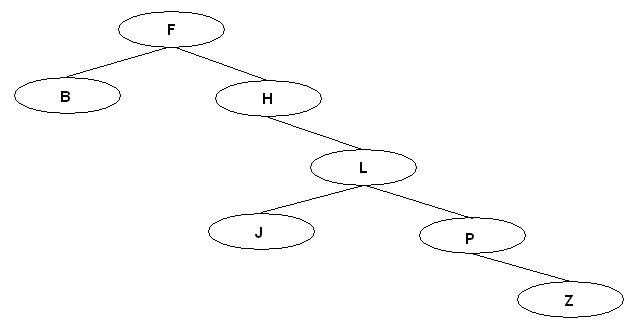
\includegraphics[width=\textwidth]{chap2/binarytree}
	\label{fig:binarytree}
\end{figure}

\section{Introductie}
Een van de simpelste zoekbomen is de binaire zoekboom. Elke interne knoop heeft twee kinderen waarvan de linkerkant lager is en de rechterkant hoger is dan de waarde in de interne knoop.\\
\\
\section{Zoeken}
Bij het zoeken naar een waarde $k$ in een binaire boom wordt begonnen in de root knoop. Als $k$ kleiner is dan de waarde in de knoop $p$ wordt verder gezocht in het linkerkind van $p$. Wanneer $k$ groter is dan de waarde in $p$ wordt verder gezocht in het rechterkind van $p$. Dit wordt gedaan tot een externe knoop is bereikt of wanneer $k$ gevonden is.\\
\\
\section{Toevoegen}
Met behulp van bovenstaande zoek methode wordt gezocht naar de toe te voegen waarde $k$. Wanneer de gevonden waarde $p$ een interne knoop is wordt er direct gestopt met toevoegen, $k$ zit namelijk al in de boom. Wanneer $p$ een externe knoop is wordt deze vervangen door $k$ en worden twee externe kinderen toegevoegd aan $k$.\\
\\
\section{Analyse}

% ********** End of chapter **********
% ********** Chapter 3 **********
\chapter{AVL-boom}
\label{sec:Hoofdstuk 3}

% ********** End of chapter **********
% ********** Chapter 4 **********
\chapter{AVL-boom}
\label{sec:Hoofdstuk 4}

% ********** End of chapter **********
% ********** Chapter 5 **********
\chapter{(2,4)-boom}
\label{sec:Hoofdstuk 5}

Intro
De tweede gebalanceerde boom die behanded wordt is de (2,4)-boom. Alle interne knopen van deze boom hebben ��n tot drie keys, het aantal kinderen van een knoop is het aantal keys + 1. Dit betekent dus dat elke knoop 2, 3 of 4 kinderen heeft, vandaar de naam (2,4)-boom (soms ook (2,3,4)-boom genoemd). Een andere eigenschap van deze boom is dat de diepte van alle externe knopen gelijk is. Deze eigenschappen zorgen ervoor dat de hoogte van een (2,4)-boom met $n$ items $\Theta(log n)$ is. Deze eigenschappen worden bewaard door na elke toevoeging of verwijdering te kijken of de boom gebalanceerd moet worden. De boom moet gebalanceerd worden wanneer een knoop in de boom geen keys (woorden) meer bevat of wanneer een knoop meer dan drie keys bevat.

Balanceren
Omdat bij deze analyse alleen gekeken wordt naar het toevoegen van keys zal de boom alleen gebalanceerd worden wanneer een knoop meer dan drie keys bevat. Wanneer een knoop meer dan drie keys bevat (overflow), zal de boom gebalanceerd moeten worden.
Dit wordt gedaan door de derde waarde van de knoop met meer dan drie keys toe te voegen aan zijn parent. De eerste twee keys worden dan het kind aan de linkerkant van toegevoegde key in de parent en de vierde waarde het kind aan de rechterkant.

Zoeken
Bij het searchen van een key zal begonnen worden bij de root knoop. Als de knoop niet de gezochte key bevat zal gekeken worden in het kind voor de key die lager is dan de invoer. Dit wordt gedaan tot een externe knoop is bereikt of tot een knoop is bereikt die de invoer bevat.

Toevoegen
Bij het toevoegen zal eerst gezocht worden op de bovenstaande manier. Wanneer een knoop wordt gevonden die de key al bevat zal gestopt worden met toevoegen. Als dit niet het geval is, we hebben dan dus een externe knoop, zal de waarde toegevoegd worden aan de parent. Hierna zal de balance methode aangeroepen worden om te kijken of de boom ongebalanceerd is en balanceren wanneer dit het geval is.

Analyse


% ********** End of chapter **********
% ********** Chapter 6 **********
\chapter{Skip List}
\label{sec:Hoofdstuk 6}

\begin{figure}[h]
	\centering
		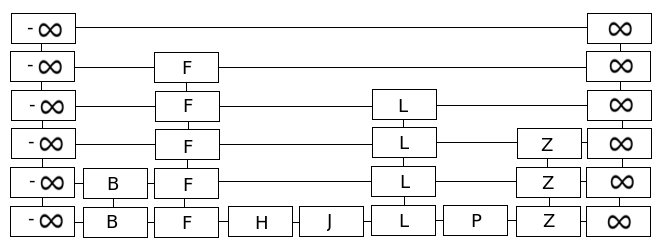
\includegraphics[width=\textwidth]{chap6/skiplist}
	\label{fig:skiplist}
\end{figure}

\section{Introductie}
Naast bomen zijn er ook andere manieren om zoekalgoritmen te implementeren. In dit hoofdsuk zal een van deze structuren behandeld worden, namelijk de skip list. Een skip list bestaat uit een aantal lijsten waarvan elke lijst een subset van de lijst onder hem bevat. De onderste lijst bevat alles waardes van de boom. Elke lijst bevat in ieder geval de waardes -\infty en \infty. Hierdoor zullen alle waardes in de lijst tussen deze twee waardes in zitten.\\
\\
\section{Zoeken}
Bij het zoeken naar een waarde $k$ in een skiplist wordt begonnen in de meest linkse waarde in de bovenste lijst, deze waarde noemen we $p$. Hierna zal gekeken worden in de waarde onder $p$, als deze niet leeg is wordt dit de nieuwe waarde van $p$. Vervolgens wordt gekeken naar de waardes aan de rechterkant van $p$. Er wordt naar rechts gezocht tot er een waarde gevonden wordt hoger dan $k$, $p$ wordt nu de waarde voor de laatst gevonde waarde. Dit wordt gedaan tot de gezochte waarde wordt gevonden. Wanneer $k$ niet in de skip list zit wordt de hoogst mogelijke waarde voor $k$ gereturned.\\
\\
\section{Toevoegen}
Bij het toevoegen van waarde $k$ wordt eerst gezocht naar $k$ op de manier zoals hierboven beschreven is. Als de gevonden waarde $p$ gelijk is aan $k$ zal direct gestopt worden, de waarde zit namelijk al in de skip list. Wanneer deze niet gelijk is zal de waarde toegevoegd worden na $p$. Hierna zal $k$ toegevoegd worden zolang een random getal tussen de 0 en 1 lager is dan 0.5.\\
\\
\section{Verwijderen}
Bij het verwijderen van een waarde $k$ zal eerst gezocht worden op deze waarde. Als de gevonden waarde $p$ niet gelijk is aan $k$ zal direct gestopt worden, $k$ zit niet in de skip list. Wanneer $k$ en $p$ wel gelijk zijn zal $p$ verwijderd worden samen met alle waardes boven $p$.\\
\\
\section{Analyse}

% ********** End of chapter **********
% ********** Chapter 7 **********
\chapter{Conclusie}
\label{sec:Hoofdstuk 7}



% ********** End of chapter **********
%%%%%%%%%%%%%%%%%%%%%%%%%%%%%%%%%%%%%%%%%%%%%%%%%%%%%%%%%%%%%
%% BIBLIOGRAPHY AND OTHER LISTS
%%%%%%%%%%%%%%%%%%%%%%%%%%%%%%%%%%%%%%%%%%%%%%%%%%%%%%%%%%%%%
%% A small distance to the other stuff in the table of contents (toc)
\addtocontents{toc}{\protect\vspace*{\baselineskip}}

%% The Bibliography
%% ==> You need a file 'literature.bib' for this.
%% ==> You need to run BibTeX for this (Project | Properties... | Uses BibTeX)
%\addcontentsline{toc}{chapter}{Bibliography} %'Bibliography' into toc
%\nocite{*} %Even non-cited BibTeX-Entries will be shown.
%\bibliographystyle{alpha} %Style of Bibliography: plain / apalike / amsalpha / ...
%\bibliography{literature} %You need a file 'literature.bib' for this.

%% The List of Figures
\clearpage
\addcontentsline{toc}{chapter}{List of Figures}
\listoffigures

%% The List of Tables
%\clearpage
%\addcontentsline{toc}{chapter}{List of Tables}
%\listoftables


%%%%%%%%%%%%%%%%%%%%%%%%%%%%%%%%%%%%%%%%%%%%%%%%%%%%%%%%%%%%%
%% APPENDICES
%%%%%%%%%%%%%%%%%%%%%%%%%%%%%%%%%%%%%%%%%%%%%%%%%%%%%%%%%%%%%
\appendix
%% ==> Write your text here or include other files.

%\input{FileName} %You need a file 'FileName.tex' for this.
\input{appendix/assignment1}
\end{document}